\documentclass[letterpaper, 12pt]{article}
\usepackage[utf8]{inputenc}

% Sane border sizes
\usepackage{geometry}

% For including images
\usepackage{graphicx}

% For multi-column stuff
\usepackage{multicol}

% Bibliography stuff
\usepackage{natbib}
\bibliographystyle{apalike}

% PDF
\usepackage{pdfpages}

%appendices
\usepackage[titletoc]{appendix}

\usepackage{amsmath}

\usepackage{enumerate}
\usepackage{listings}

\usepackage[normalem]{ulem}
\useunder{\uline}{\ul}{}
\lstset{
    %frame=tblr,
    framesep=5pt,
    %basicstyle=\tiny,
    showstringspaces=false,
    keywordstyle=\itshape\color{blue},
    identifierstyle=\ttfamily,
    stringstyle=\color{Maroon},
    commentstyle=\color{black},
    xleftmargin=5pt,
    xrightmargin=5pt,
    % aboveskip=\bigskipamount,
    % belowskip=\bigskipamount,
    %backgroundcolor=\color{LightGray!.50}
}

\numberwithin{figure}{section}%for figures
\numberwithin{table}{section}%for tables

% Don't let figures in one section go into the next section
\usepackage[section,subsection,subsubsection]{placeins}

% THE DOCUMENT BEGINS HERE
\begin{document}

% Document-wide length definitions go here

% Space between paragraphs
\setlength{\parskip}{\baselineskip}

% bigskip is not big enough
\newskip\bigskipamount   \bigskipamount =42pt plus 4pt minus 4pt


\begin{titlepage}
\begin{center}

{\Large
    \textsc{Visualization and Simulation of CBMS Dataset}
\par}


\bigskip
A Technical Manual\\
Presented to\\
the Faculty of the College of Computer Studies\\
De La Salle University

\bigskip
In Partial Fulfillment\\
of the Requirements for the Degree of\\
BS Computer Science with Specialization in Software Technology

\bigskip
by

Base, Jhonn Jelvin S.\\
Calulo, Lawrence Patrick C.\\
Co, Bervyn S.\\
Lo, Charles Geoffrey R.

\bigskip
Dr. Nelson Marcos\\
Adviser

\bigskip
\today

\bigskip
\date{today}
\end{center}
\end{titlepage}



\tableofcontents
\clearpage

% Start counting pages at the research description
\setcounter{page}{1}
\pagenumbering{arabic}


% INCLUDE CHAPTERS HERE

\section{Overview}

\textbf{ComStat} is a web application designed to be used as a tool for visualizing and simulating Community-Based Monitoring System (CBMS) data. Users can upload datasets, provided as CSV files compressed into ZIP or
CAN\footnote{CBMS's CAN files are in fact ZIP files with a different extension.}
files

The system is built as a client-server system: the server is written in Python, built with Django and exposing a
RESTful\footnote{\textbf{Representational State Transfer}, which is essentialy a set of specific semantics that map to HTTP methods.}
API; and the client is written in JavaScript, built with AngularJS, and consumes the API.


\subsection{Essential terminology}

\begin{itemize}
    \item \textbf{Back end.} This refers to the Python components of the system, responsible for storing dataset data, computing simulations, and serving data to the front end through the API. The Django framework, and related libraries, are used for this part.
    \item \textbf{Front end.} This refers to the JavaScript and HTML components of the system, which runs on the user's Web browser. This is responsible for displaying the user interface through which users interact with the system. The Angular framework, and related libraries, are used for this part.
    \item \textbf{Application Programming Interface (API).} Refers to the URLs located under \texttt{/api/} through which the front end interacts with the back end.
    \item \textbf{Main CSV.} For the purpose of this system's technical discussion, this refers to the CSV file containing one entry for every household containing information such as interview date and household GPS coordinates. CBMS data files usually have \emph{HH} or \emph{main} in the file names of their main CSV files.
\end{itemize}


\subsection{Prerequisite technical knowledge}

The system is expected to handle the data of hundreds of thousands of households while staying within reasonable and practical limits for memory usage and processing time. As such, some features specific to the particular technology choices for the system are used.


\subsubsection{Python}

The system uses Python 3, and as such a casual familiarity with the specifics of this version of Python is expected. In particular, an understanding of Python 3's distiction between \texttt{string} and \texttt{byte} data types will be helpful when working with the Dataset Management module.

\emph{Generators} are another important feature that gets used in the system's code. It gets used by the Simulation module code as an easy way to iterate over a large amount of household data without creating duplicate arrays for that data. A simple generator example is as follows:

\begin{lstlisting}

def do_something(things):
    for thing in things:
        # <some processing happens here>
        yield thing

\end{lstlisting}

Simply put, the above Python function iterates through the given \texttt{things}, returning an iterable generator object with the \texttt{yield} keyword. Because the Simulation module's code is composed of multiple steps, ranging from retrieving households from MongoDB to attaching metadata to the household records, this pattern is seen in many functions in this module.

Lastly, the back end relies heavily on unit tests to verify that key pieces of code return the correct results. These tests are located under the \texttt{tests} folder inside each Django app's folder\footnote{For example, \texttt{datasets/tests/} or \texttt{api/tests/}}. It is \textbf{very strongly recommended} that the code is maintained such that the tests always pass, to ensure that no existing system functionality breaks during future development. It is also strongly recommended that further development also rely on unit tests to allow for easy and confident refactoring, as well as to provide assurance that further development produces code that does exactly what is intended.


\subsubsection{JavaScript} 

Angular is used as a framework for building the front end. Its data binding functionality enables the easy synchronization of interface and underlying data model. Angular's \emph{directives} allow the packaging of UI components and logic into custom-made reusable tags. The related library \emph{UI Router} allows for rapid reload-free transitions between different pages of the application. As such, it is necessary to acquire at least a basic understanding of these features in order to work on the ComStat front end. Details on all of the aforementioned can be found in their respective pages on the Internet.

Like the back end, the front end also comes with unit tests. However, these were abandoned during development. However, should it become desirable to have a suite of unit tests for the front end, the old tests can act as a springboard from which further tests can be patterned after.

% \emph{ComStat} is a web application that visualizes and simulates CBMS (Community Based Monitoring System) data that can be used ideally using Google Chrome as its browser. The system aims to give city officials as well as researchers a platform for visualizing a desired indicator. In effect, the system provides a representation per household and the color of the representation represents how good or bad is the households in a desired field. The system can accept two types of users. These are an admin, which has a complete enabled features, and a non-admin user, which is a restricted type of user.

% As an admin user, he/she is entitled complete working features for the system. He/she can add new dataset, edit his/her own dataset and delete its own dataset. After creating his/her own dataset, the user upload his data in a .ZIP or .CAN file. After uploading, the user should process the data by filling up the necessary fields, or an auto-complete button. After processing, he/she can either upload a metadata, upload shape files, extract and download, visualize the data uploaded and simulate the data by using basic mathematical formula.

% On the other hand, if a user is not an advanced user, he/she needs to ask for an access of the dataset he/she wants to use for visualization and simulation.

\clearpage


\section{Dataset Management Module}

The Dataset Management Module is responsible for storing, keeping track, and retrieving data. To achieve this, both MongoDB and PostgreSQL are used.

\begin{itemize}
\item \textbf{PostgreSQL} is used for storing bookkeeping data. This includes the dataset name, references to metadata files, field types, and the like. This data naturally fits in the relational paradigm of data storage.
\item \textbf{MongoDB} is used for storing data from uploaded CSV files. This data can be highly variable in terms of schema, making this a natural fit for a document-oriented data store.
\end{itemize}


\subsection{Bookkeeping}

The Django Object-Relational Mapper (ORM) is used for modelling bookkeeping data and interacting with the PostgreSQL for persistent storage.

\section{Map Visualization}
The Map Visualization part of the Visualization module is a part of the system that allows a user to visualize data through geographic maps upon choosing the field in the data. The module uses different libraries: 
\begin{itemize}
	\item \textbf{Google Maps API}
	This library is being used for visualizing data through geographical maps. Images that are rendered on visualization are supported by Google Maps API library. 
	\item \textbf{D3.js}
	This library implements the numerical and non-numerical 2-variable visualization. After the user selected two fields that are numerical and non-numerical(metadata should be uploaded), the library will render donut marker that represents per household. Since non-numerical fields generate randomize color and Google Maps API doesn't support rendering donuts. D3.js is used. 
	
	\item \textbf{Angular Range-Slider}
	This library implements the two-handler slider that simulates future status per household. Instead of having one-handler slider that has fix minimum and adjustable maximum, two-handler slider is implemented. It allows the user flexibility on having an adjustable minimum and maximum and also visualizes the household inside the adjusted minimum and maximum. 
	
	\item \textbf{Chroma.js}
	This library is needed to generate colors for non-numerical items. Colors can range from orange, yellow, blue, indigo and violet. Red and green colors are not allowed since it might confuse the user non-numerical to poverty indicator formula.
\end{itemize}
\subsection{Household Level}
Household level visualization is one of the feature of this module. Using the Google Maps API and D3.js, the user can visualize one to two fields selected by the user. By determining the color appropriate for a certain household because of his/her status, marker is rendered with a custom image as its icon. Rendering a custom icon is important because it lessen the stress of the system if thousand or millions of the data are needed to be visualized. Numerical and non-numerical visualization are not handled by Google Maps API because of the randomize color used by non-numerical field. D3.js handles that situation. D3.js handles the visualization of the numerical and non-numerical 2 variable visualization.

\subsection{Barangay Level}
Barangay level visualization uses Google Maps API also as its main library. The user can visualize all barangays or selected barangays. By converting the shape files into GEOJSON format and uses the Google Maps API for map setting and style or coloring of the polygons. 

\subsection{Simulate Data Through Sliders}
Simulating the household data through sliders is handled by ``Angular Range-Slider" library. It gets the adjusted minimum and the adjusted maximum through sliding the handler from left to right or vice-versa. In effect, this will show how the household is performing if the threshold is changed from time to time.

\clearpage

\section{Chart Visualization}

The Chart Visualization is a part of the system that allows the user to create charts as a form of visualization upon choosing the field in their data. The module uses Google Charts API to generate the necessary charts needed for visualizing data.

\begin{itemize}

\item \textbf{Google Charts API} is the library that is being used for visualizing data in the form of charts. While using the library, requests are being thrown to the API online. 

The charts that are available in the library include bar chart, column chart, histogram, pie chart, donut chart, scatter chart and line chart. 

\item \textbf{Google ChartEditor Package} is a package that is included in the Google Charts API that lets the user edit and change the style of the map. It allows the user to change the chart title, chart color and modify legends among others. It also allows user to change between different charts.

\item \textbf{Downloading Charts} is possible within the visualization module. Using the Google Charts API, the user can download the chart that is generated when a field in the data is chosen. A request is thrown to the API and sends back a PNG format of the chart that can be downloaded.

\end{itemize}

\clearpage


\begin{appendices}

\section{ERD/Class Diagram}

All interactions with the relational database are done via the Django ORM. Furthermore, because the exact data type in the database is dependent upon which database is used (which, currently, is PostgreSQL) the Django ORM data type is listed instead.

Also, because Django converts the Python \texttt{None} value to an empty string before saving it into \texttt{CharField} and \texttt{TextField}s, these fields are marked as nullable although they are not nullable at the database level.

\begin{figure}[h!]
    \centering
    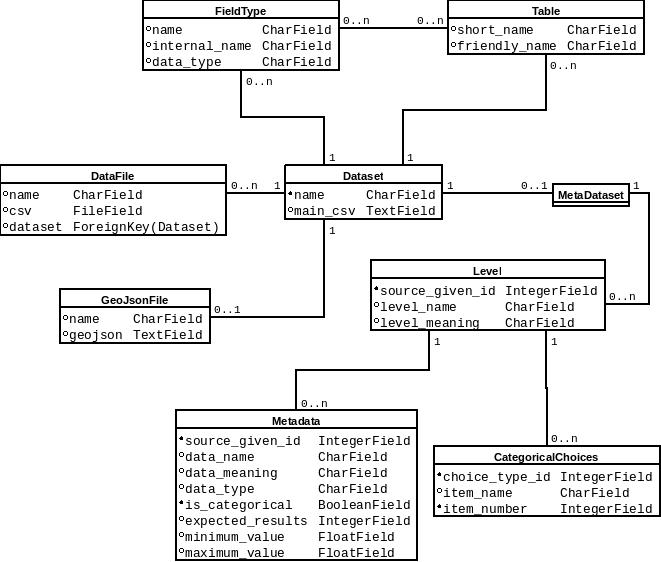
\includegraphics[width=120mm]{images/erd.jpg}
    \caption{The entity relationship diagram (ERD) for ComStat's ORM classes}
    \label{fig:img-comstat-erd}
\end{figure}

\end{appendices}

% \bibliography{references}
\end{document}
